\section{Data Acquisition (DAQ)} 
\label{sec:daq}

%%%%%%%%%%%%%%%%%%%%%%%%%%%%%%%%%%%%%%%%%%%%%%
\subsection{Scope and requirements}

This section outlines the data acquisition (DAQ) for ProtoDUNE-SP.
The DAQ system is shown in figure \ref{fig:daq-overview} along with its
interfaces to the cold electronics, beam instrumentation, and online
computing systems.


\begin{cdrfigure}[DAQ Overview]{daq-overview}{Detailed overview of the
DAQ system, its interconnections, data flow, timing and control signals,
and the interfaces to the electronics and online computing systems}
        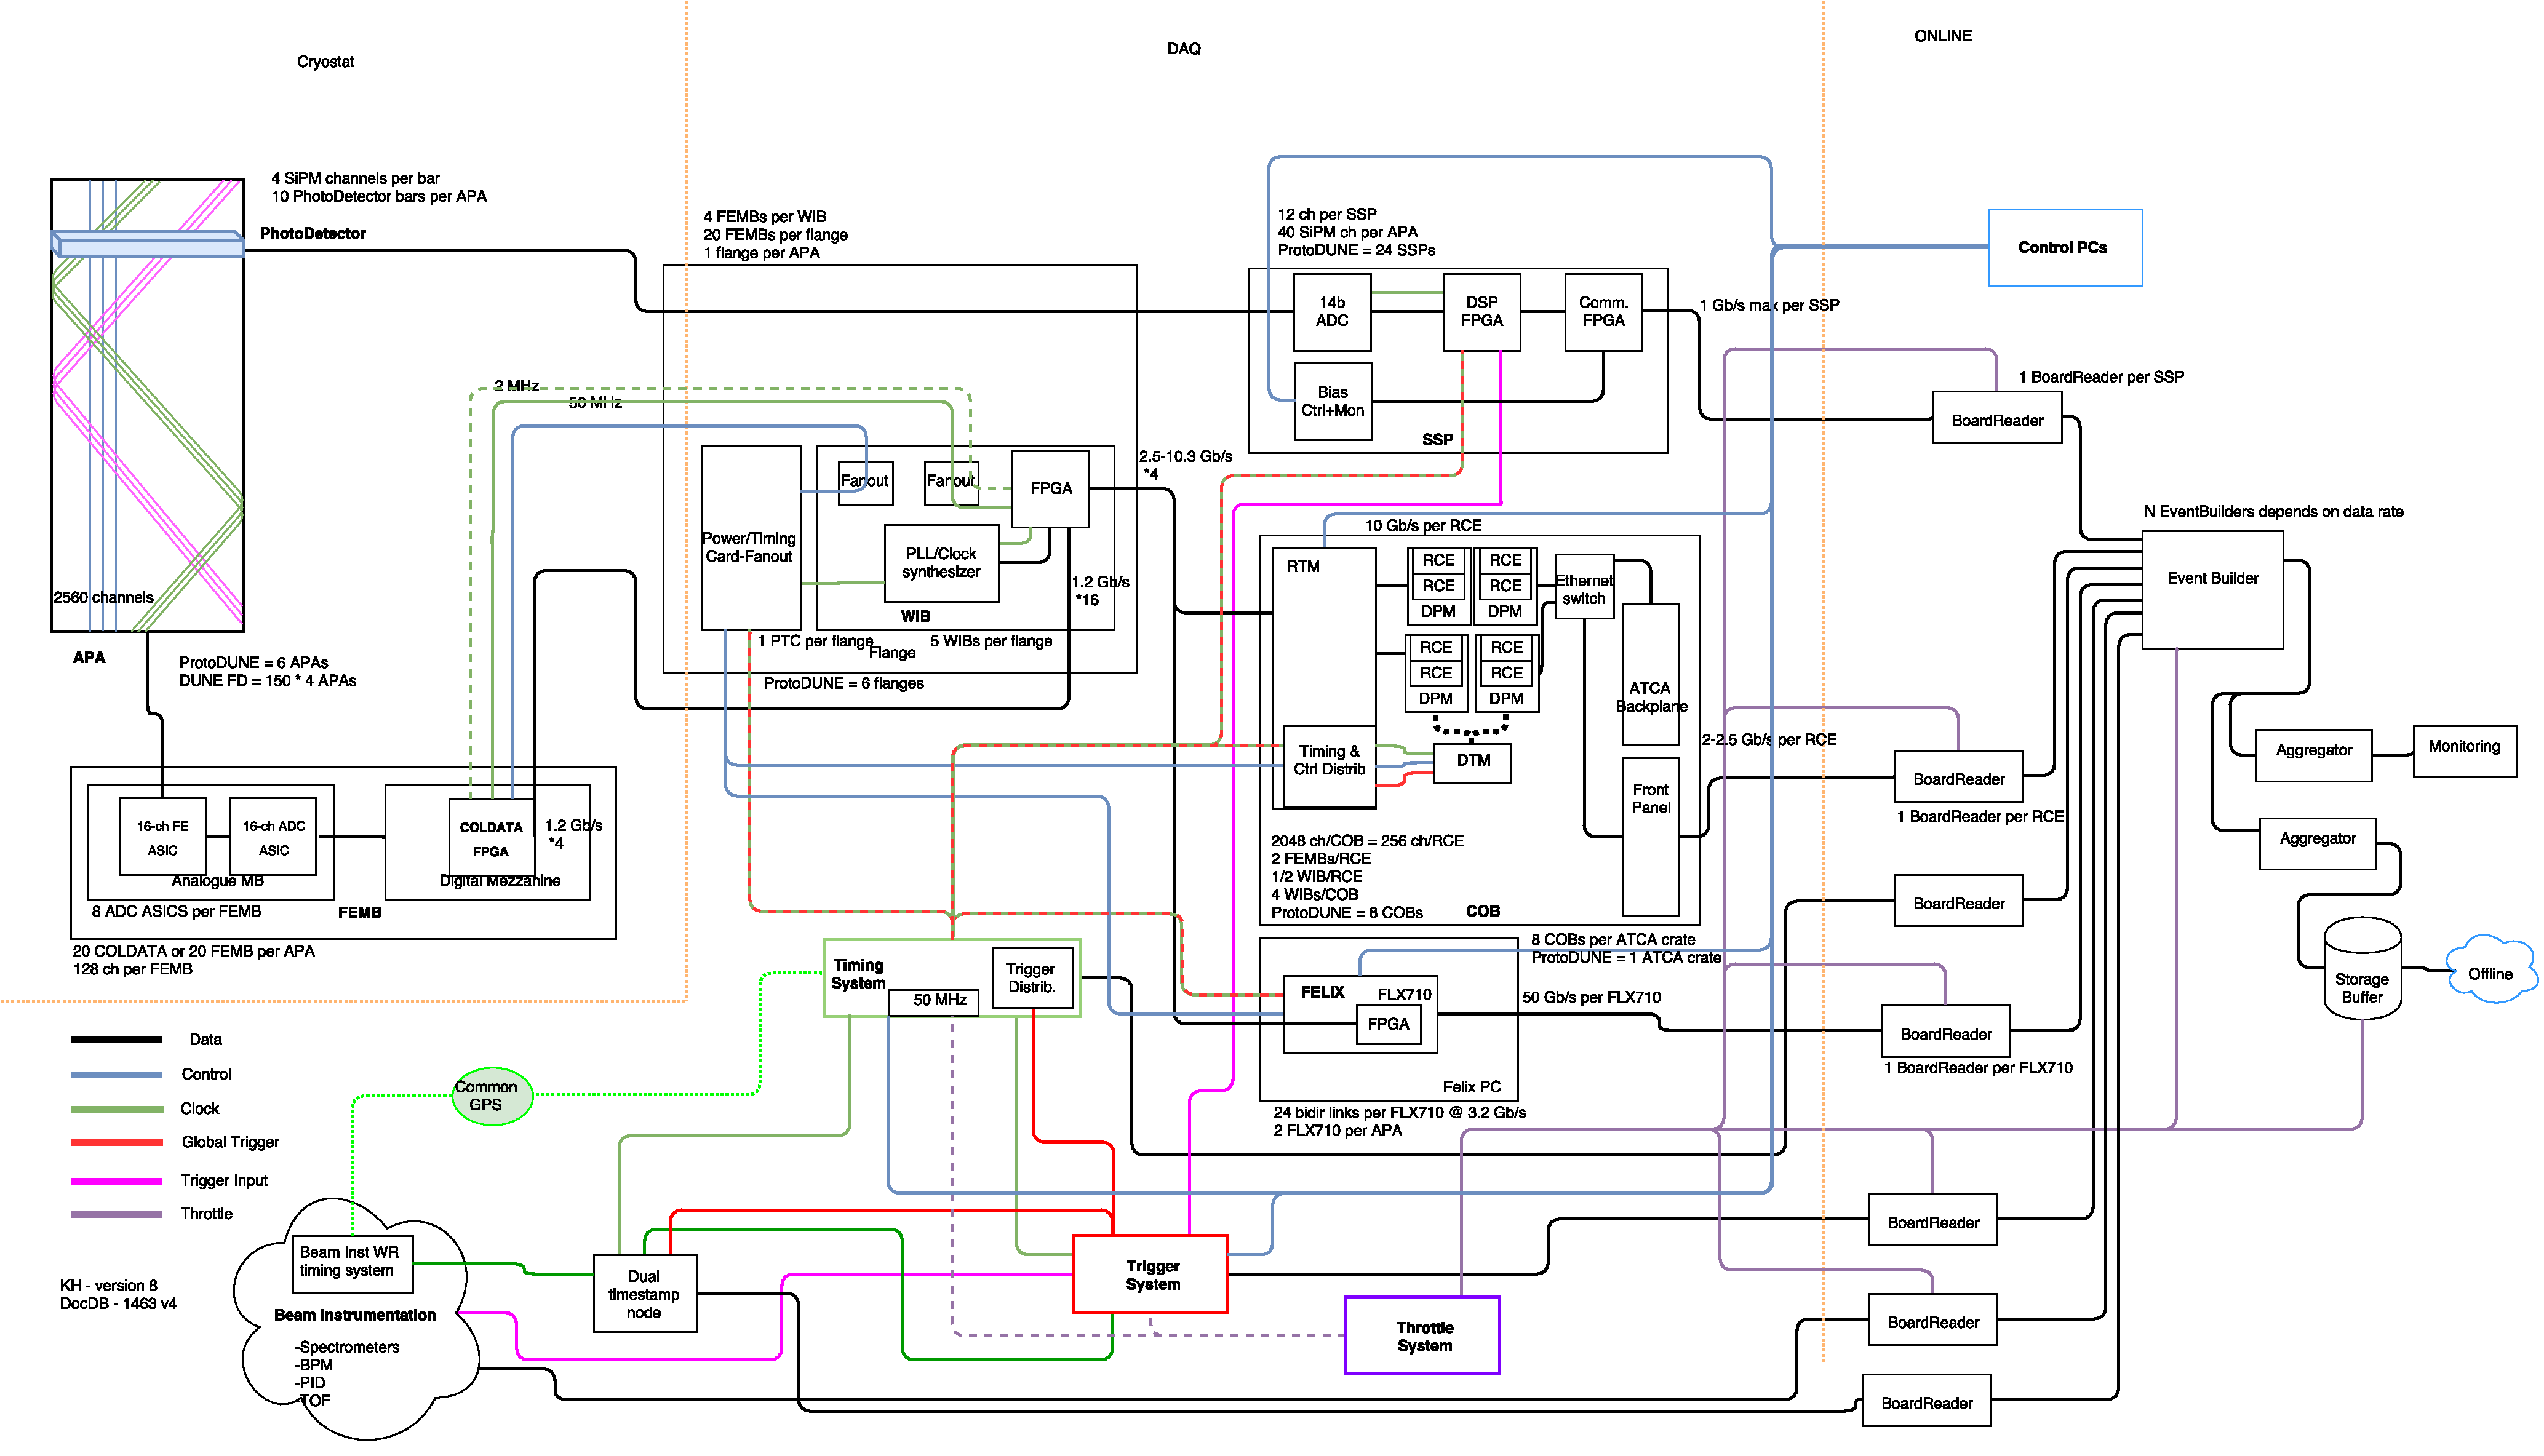
\includegraphics[angle=90,width=0.70\textwidth]{daq-overview-dia.pdf}
\end{cdrfigure}

The requirements for the DAQ system for ProtoDUNE-SP are defined
by the physics requirements of the experiment, with constraints from the
front-end electronics and assumed bandwidth and storage requirements
from the online and offline computing systems.  The baseline trigger
rate during the SPS spill is taken to be 25 Hz.  Cosmic data will also
be acquired at an appropriate rate such that bandwidth and processing priority are given 
to beam data.

The data rate from the electronics will be dominated by the
TPC data.  However, the photon detection system (PDS) can produce a signifcant
amount of calibration data (where full waveforms are extracted), during
commissioning and special runs (up to 24 Gb/s maximum).

The TPC data is sent via the Warm Interface Boards  (WIB) on the cryostat flanges
for the six APAs of ProtoDUNE-SP, un-triggered at a total rate of 480 Gb/s
.  The PDS data is estimated to send data
at a total rate of 1.2 Gb/s from the 24 SSPs (detailed further in subsection \ref{subsec:pds-readout}).
The maximum bandwidth from the ProtoDUNE-SP online system to CERN IT (and
hence, the offline world), is 20 Gb/s at a maximum.
Therefore, the DAQ system must reduce the data by a significant fraction
before it is sent offline.  This is achieved by a combination of
data compression and triggering.


%%%%%%%%%%%%%%%%%%%%%%%%%%%%%%%%%%%%%%%%%%%%%% 
\subsection{Timing, trigger and beam interface}
\label{sec:daq_time}

The timing and the trigger are two distinct subsystems.  The timing
system provides the distribution for the trigger signals over the same
fabric as the clock and calibration signals.  Each of the systems will
be described separately, along with a brief section on the interface to
the beam instrumentation.

\paragraph{Timing}


The timing system is required to: provide a stable and phase-aligned
master clock to all DAQ components; synchronize external signals into the
ProtoDUNE-SP clock domain and time-stamp them; distribute synchronization,
trigger and calibration commands to the DAQ system; and conduct continuous
checks of its own function. In addition, the timing system acts as a
data source, providing a record of triggers received, distributed, or
throttled. The system is designed to meet the full eventual requirements
of the DUNE experiment, but will need only a subset of that functionality
for ProtoDUNE-SP. For instance, absolute time-stamping with respect to an
external GPS reference is not required.

An FPGA-based master unit receives a high-quality clock (from a quartz crystal oscillator or external source) 
and external signals from the
trigger system and SPS accelerator. It interfaces to the ProtoDUNE-SP control
and DAQ via a gigabit Ethernet interface. The master unit multiplexes
synchronization and trigger commands, along with arbitrary command
sequences requested by software, into a single encoded data stream,
which is broadcast to all timing endpoints, and decoded into separate clock
and data signals. A uniform phase-aligned cycle counter, updating at the
ProtoDUNE-SP system frequency of 50MHz, is maintained at all endpoints,
allowing commands to take effect simultaneously at all endpoints
regardless of cable lengths or other phase delays.

The timing signal is broadcast via multi-mode optical fiber (for
medium-distance connection to the WIB crates on the detector) and LVDS
signals over twisted pair cable (for short-distance connection to RCEs,
SSPs and FELIX modules). Optical signals are fanned out and recombined
using commercial 32:1 passive splitters, and active optical--LVDS
converter boards further split the signals for local distribution to
endpoints. 

Endpoints decode the timing signal into separate clock and data
signals using a commercial clock-data recovery ASIC \cite{siliconlabs:Si5344}, which in turn
feeds a low-bandwidth PLL in order to remove any remaining jitter in
the clock and provide phase adjustment. The data stream employs 8b/10b
encoding, ensuring sufficient transitions in the timing signal for clock
recovery and correct operation of optical links, and uses scrambling
of idle patterns to minimise ElectroMagnetic Interference (EMI).
 A common firmware block is used to
decode the timing protocol, which is incorporated into the overall
firmware design for the receiving FPGA in each DAQ component. This
block provides a cycle counter, several independent trigger, calibration and 
synchronisation signals, and a general-purpose packet data output to each endpoint.
The cycle counter is used to generate low-frequency timing signals for
further propagation, e.g. the 2MHz sampling signal for the cold ADCs.

\paragraph{Trigger}

The baseline trigger solution for ProtoDUNE-SP is the Central Trigger Board
(CTB). The CTB is designed to receive triggers from various sub-systems
(Photon Detection System, Beam Instrumentation, SPS spill signal, veto
signals, etc.).  Up to 100 input channels are provided.  It combines
these into a global trigger based on a configurable input mask (or
more sophisticated algorithm if desired).  It provides functionality
to globally time-stamp triggers, keep event counts, and provide artDAQ
compatible header information with trigger type and error conditions.
Internally generated triggers and calibration pulses allow for testing
the board itself and the end-points receiving the trigger signals.

The CTB is based on the MicroZed development board \cite{avnet:microzed}, which comprises a
Xilinx Zynq-7000 System-on-Chip (SoC), 1 GB DDR3 RAM, Gigabit Ethernet,
and 115 I/O ports.  The Programmable Logic of the Zynq-7000 is used to
perform fast triggering operations, whilst the Processing System is used
to interface to the readout and controls systems.

Configuration and operation is performed using an XML file which is sent
to the CTB.  This allows for fast reconfiguration of the CTB without
the need for new firmwares.  The file is used to both configure the board
and send start/stop/reset/etc. commands from the run control.
The trigger output format for ProtoDUNE-SP consists of a trigger type (physics/calibration/random),
a time-stamp, the trigger word, counter information and the values 
of the inputs causing the triggers.  
The trigger system will use the timing system clock and global triggers will be
distributed via the timing system.  


\paragraph{Beam Interface}

The Beam Instrumentation is described in detail in section \ref{sec:beaminstruments}.
The beam instrumentation data acquisition and the data acquisition for ProtoDUNE-SP
will have separate timing systems.  A common GPS clock will be used to keep both
systems synchronized relative to each other.  A common endpoint will receive time-stamps 
from both WhiteRabbit (for the beam instrumentation) and the ProtoDUNE-SP timing system
will be used to create a matching table from the two systems.  Data from the beam
instrumentation will be acquired continuously via a separate DAQ path.  Triggered
data for ProtoDUNE-SP will have both the TPC, PDS, and beam instrumentation data and 
the timestamps and trigger information of both.

%%%%%%%%%%%%%%%%%%%%%%%%%%%%%%%%%%%%%%%%%%%%%% 
\subsection{TPC data readout}

The readout of the ProtoDUNE-SP TPC wires, prior to being received by PCs in
the back-end DAQ, consists of  electronics directly attached the APAs,
inside the cryostat (the cold electronics, CE) and  electronics outside
the cryostat, both directly on the cryostat flange and in a rack (the
warm electronics).  This subsection
addresses the warm part of the TPC
readout and how it receives data from the cold electronics (the Front-End
Boards), manipulates the data, and delivers it to the back-end DAQ.

From an electronics point-of-view, the ProtoDUNE-SP flange will consist of
5-slot ``crate'', where the connectors on the warm side of the feed
through form the ``back-plane'' into which the boards plug when inserted
into the ``crate'' assembly.  These connectors and the boards that plug
into them (the WIBs, or warm interface boards) serve to send the power,
timing, and configuration down to the FEBs and receive the high-speed
signals from the FEBs. From a data standpoint, each WIB receives the
data from 4 FEBs, over sixteen 1.25-Gbps data lines, and multiplexes
this data to four 5-Gbps (or two 10 Gbps) lines which are sent over
optical fiber to the DAQ.

Two systems will be used to receive data from the WIBs.  The baseline
solution is based on Reconfigurable Computing Elements (RCE) and will
readout data from 5 APAs.  An alternative exploratory prototype based on
the Front-End-Link-EXchange (FELIX) system will be used to readout 1 APA.

\paragraph{RCE-based readout}
The data from the WIB are received by processing units called RCEs (Reconfigurable Cluster Element), 
\cite{slac:rce}
which are housed in industry-standard
ATCA shelves on COB (cluster-on-board) motherboards that are designed
at SLAC for a wide range of applications.   The RCE is a SoC 
from the
Xilinx Zynq family and contain a full Linux processor system on the chip
accompanied by 1 GByte of DRAM.   The primary processing function of the
RCEs for ProtoDUNE-SP are compression (and/or zero-suppression) and buffering
of the raw data and then sending data to the back-end upon the receipt of
an external trigger.  Each COB carries 8 RCEs, all connected to each
other via an on-board 10 Gbps Ethernet switch which also sends data out
of the COB to the back-end DAQ PCs.

The interface with the WIB is provided via the ATCA compliant rear-board, the RTM (Rear Transition Module).  
For ProtoDUNE-SP, this application-specific board will use a set of QSFP transceivers to receive
the data from the WIB and an SFP+ (small form-factor pluggable)
 optical interface for communication
with the timing and trigger distribution system.

As the multiplexed data from the WIB comes into the RCE FPGA fabric
it will be de-multiplexed and buffered into per-channel, fixed-time
length chunks (for instance 512- or 1024-ticks).  These chunks will be
compressed and written to the DRAM where the RCE processor will wait
for a trigger (also handled by the FPGA) to arrive.  Upon a trigger, the
processor will send data for a fixed window in time, including pre- and post-trigger time chunks,
for all channels, to the back-end PCs.  

For ProtoDUNE-SP, 256-wires worth of data (2 FEBs) will be sent to each RCE.
Given that there are 120 FEBs in ProtoDUNE-SP, 60 RCEs will be needed to
readout the full detector.  These will fit into 8 COBs which in turn
will reside in a single 14-slot ATCA shelf.

\paragraph{FELIX-based readout}
The FELIX is a PCIe card receiving data on point-to-point links from
the detector electronics and routing those through a switched network
to computers.  The aim is to reduce to a minimum any specific hardware
developments and to fully rely on commercial networks and servers to
perform the DAQ tasks.  For ProtoDUNE-SP, data from 5 WIBs (20 FEBs) will
be readout over ten 9.6 Gbps links into two FELIX cards.  Grouping
time-slices around a trigger signal, as well as data compression will be
dealt with in software. Similar to the RCE based readout the FELIX will
generate artDAQ fragments to be sent to the event builder.


%%%%%%%%%%%%%%%%%%%%%%%%%%%%%%%%%%%%%%%%%%%%%% 
\subsection{PDS and beam instrumentation data readout}

\paragraph{PDS readout} 
\label{subsec:pds-readout}
The PDS data rates are described here.  The PDS electronics and DAQ are
described in section \ref{sec:pds-elec-daq}.  The plan for PDS data
readout is as follows.  A combination of externally triggered events
and self-triggered events will comprise the data.  The external triggers
will come from the beam instrumentation via the trigger system at 25 Hz.
This amounts to 118 Mb/s.  The self-triggered data
will be induced by cosmic rays.  A cosmic rate of 10 kHz is assumed,
totalling 1106 Mb/s.
The combined rate comes to $\approx$1.2 Gb/s.  An alternative scheme with
just self-triggered header-only data is considered for implementation if
the former proves difficult; with a resultant rate of $\approx$1.1 Gb/s.


%%%%%%%%%%%%%%%%%%%%%%%%%%%%%%%%%%%%%%%%%%%%%% 
\subsection{Event-building software }

Developed within the Fermilab Scientific Computing Division and
already used for the LBNE-35ton prototype, artdaq provides data
transfer, event building, and event analysis functionality. This
latter feature includes built-in support for the art event analysis
framework \cite{fnal:art}, allowing experiments to run art modules for real-time
filtering, compression, disk writing and online monitoring. As art,
also developed at Fermilab, is also used for offline analysis, a major
advantage of artdaq is that it allows developers to easily switch
between developing online and offline software.

There are three types of processes provided by artdaq, each of which
fulfills a specific role; in order of upstream-to-downstream, these
are boardreader processes, eventbuilder processes, and aggregator
processes. A given boardreader process is intended to be associated
with a particular geographical region of the detector, and provides
hooks (in the form of C++ base classes) for an experiment's developers
to embed experiment-specific code (called ``fragment generators'')
designed both to upload configuration values to hardware and to read
out the hardware. For ProtoDUNE-SP, the full DAQ will consist of 87+ 
boardreaders, in charge of the 60 RCEs, 24 SSPs, the timing system, 
the Penn Trigger Board, and at least one for the beam instrumentation.
%For testing purposes whenno hardware is available, fragment generators are available whichdon't actually interface to true hardware, but instead perform usefulfunctions such as read in existing output files, extract theirfragments and send them downstream (serving as a "playback" mechanism,essentially) as well as model pathological behavior such as sudden,precipitous increases in data rate or unexpected dropoffs in upstreamdata flow.  (Shorten per Eric J)
For testing purposes, fragment generators can perform useful
functions such as providing a ``playback" mechanism,'' and modeling sudden or unexpected data flow events.

Downstream of the boardreader processes are the eventbuilder
processes. An eventbuilder receives data from every boardreader (a
chunk of data from one boardreader corresponding to an event is
referred to as a "fragment"), and assembles the fragments for a given
event into a raw, complete data event. Optionally, filtering via art
modules can be performed at this stage.

The most downstream process type is the aggregator. Traditionally in
artdaq-based DAQ systems, there are two aggregators, one in charge of
writing data to disk and reporting aggregate statistics (MB/sec,
e.g.), and one in which experiments can run art analysis modules for
real-time online monitoring. 
%
%For ProtoDUNE-SP this model will change asartdaq becomes more flexible; current versions of artdaq supportmultiple diskwriting aggregators which may increase throughputcapability as well as support for multiple monitoring processes whichare decoupled from artdaq. It is possible for much of the functionalityof aggregators to be replicated in eventbuilders; while this reducesthe number of interprocess connections in the DAQ software, adisadvantage of an eventbuilder-only system is that the number ofprocesses assembling raw events is the same as the number of processeswriting to disk.
%
For ProtoDUNE-SP this model will change as
artdaq becomes more flexible and throughput
capability increases. The functionality
of aggregators may be replicated in eventbuilders. While this solution  reduces
the number of interprocess connections in the DAQ software, the number of
processes assembling raw events is the same as the number of processes
writing to disk.


%For the 35ton prototype, artdaq processes were controlled by a program calledDAQInterface. DAQInterface can be thought of as an intermediarybetween Run Control and the individual artdaq processes; it's incharge of launching the artdaq processes and sending themconfiguration code on initialization, and repeatedly querying theprocesses to see whether or not they return an "Error" state; if thisis the case DAQInterface will automatically stop datataking and shutdown the processes in an orderly fashion, so that unexpected behaviorfrom upstream (e.g., hardware suddenly sending an unmanageably highrate of data) will not result in improperly closed output files,zombie processes, etc. For ProtoDUNE-SP, the plan is to shift some of the functionality of DAQInterface (such as querying artdaq process status) over to JCOP (Joint Controls Project); where appropriate/possible, DAQInterface code will be reused so as to minimize unnecessary duplication of effort. 
 
For the 35-t prototype, artdaq processes were controlled by a program called
DAQInterface. DAQInterface takes 
charge of launching the artdaq processes, checking for error states, and
shutting down
 processes in an orderly fashion as needed, to avoid improperly closed output files,
zombie processes, etc. For ProtoDUNE-SP, some of the functionality of DAQInterface (e.g., querying  status) will shift to JCOP (Joint Controls Project);
DAQInterface code will be reused as appropriate/possible, to minimize duplication of effort. 



%%%%%%%%%%%%%%%%%%%%%%%%%%%%%%%%%%%%%%%%%%%%%% 
\subsection{Control, configuration and operational monitoring}

The artDAQ software used for all applications dealing with the movement,
processing and storage of data will be interfaced with software of the
Joint Controls Project (JCOP) for the purpose of control, configuration
and operational monitoring.  JCOP provides a toolkit to implement run
control (finite state machine (FSM), distribution of commands, error
propagation and handling) as well as graphics tools that allow for the
implementation of user interfaces and monitoring dashboards.  In order to
minimize the software development needs the same FSM as defined by artDAQ
will be implemented and commands will be sent to the applications using
the already supported XML-RPC protocol.  Monitoring data will be pushed
into the JCOP framework by implementing the appropriate artDAQ monitoring
plugin.  Log and error messages will be most probably collected and
processed using an implementation of the ELK (elastic search, logstash,
kibana \cite{elastic:kibana}) stack. 
 The internal configuration of DAQ applications will be
carried out using the mechanisms provided by artDAQ. The overall system
will be modeled and configured using the JCOP paradigm (data points).


%%%%%%%%%%%%%%%%%%%%%%%%%%%%%%%%%%%%%%%%%%%%%%
\subsection{Data-quality monitoring}

In addition to the monitoring of the operations of the DAQ system, the
quality of the data taken by the detectors has to be constantly monitored.
This assurance is provided by the online and nearline monitoring systems.
This subsection describes the baseline monitoring frameworks for ProtoDUNE-SP.  
The final implementation is subject to change, but will likely be similarly
linked to artDAQ and LArSoft as described here.

\paragraph{Online monitoring}
The Online Monitoring framework will run as a DAQ process and therefore be
able to provide data quality assurance in real-time. artDAQ will split the  
data into distinct physics and monitoring streams via its aggregator processes.  
The data rate to the monitoring will be tunable such that the monitoring 
can digest the data in a timely fashion.
The software framework used for online monitoring 
%shown in Figure~\ref{fig:OnlineMonitoringFramework}.  It 
consists of an
\texttt{art::Analyzer} module which interfaces with the artdaq framework and
owns instances of further classes, each designed to handle different aspects
of the monitoring.  
%\fixme{whatever the current baseline is should be described as the ProtoDUNE-SP default; where apronpriate it is fine to also describe alternates; as written it appears that we don't know what the system will look like for ProtoDUNE-SP which is not good. }

%\begin{cdrfigure}[Online Monitoring software framework]{OnlineMonitoringFramework}{
    %Class diagram showing the baseline online monitoring framework. 
    %\fixme{This figure may be too detailed and specific when the text seems to suggest that we don't quite know yet what things will look like. Consider to make less technical and show idea and fewer details }
    %}
  %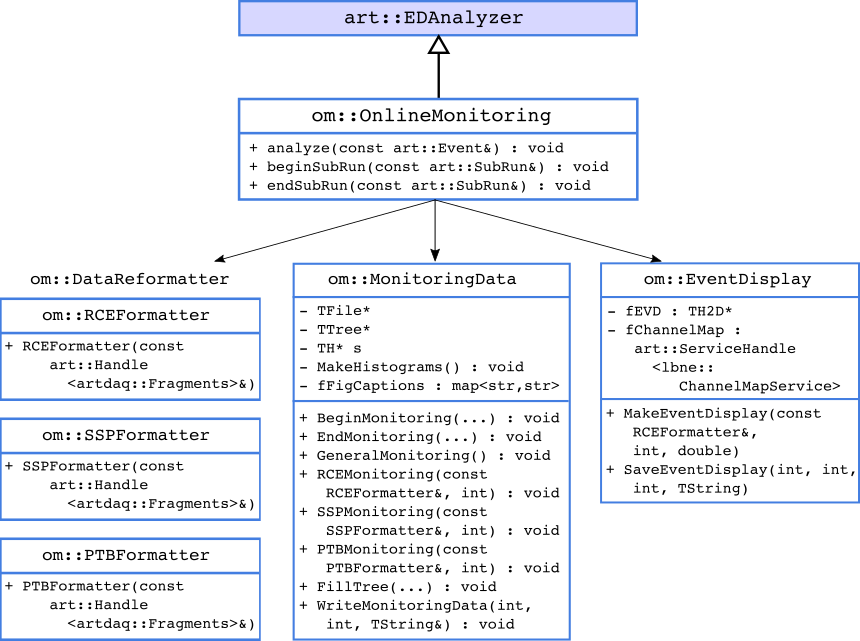
\includegraphics[width=0.8\textwidth]{online_monitoring_software.png}
%\end{cdrfigure}

The DataReformatters restructure the data to allow for efficient subsequent
analysis and provide a standard interface to the methods which look through
the events.  These reformatted objects are passed to MonitoringData, which
owns all of the data products (\texttt{TTree}s, \texttt{TH1}s, \texttt{TGraph}s
etc.) output from the monitoring software and provides methods for filling
them when required.  Finally, the online event displays are
written as part of the monitoring framework, so the EventDisplay class was
responsible for this.  
%This particular functionality will possibly be handled
%differently in ProtoDUNE-SP.
%\fixme{same comment as above - this is not a 35t detector TDR}

The output is then saved in a common area for offline access and for syncing
with a web server. This will be hosted at CERN and will allow for remote
monitoring of the experiment.

\paragraph{Nearline monitoring}

The Nearline Monitoring is designed to provide complimentary information to
that given by the online system. It runs separately as a series of automated
shell scripts and provides feedback on a slower timescale than the online
monitoring, thus allowing for a broader view of the quality of data over time.
It also utilises offline software (LArSoft) to provide, for example,
reconstruction, facilitating a more complete monitoring of much more complex
information.

Once an output data file has been closed by the DAQ, it can be processed by the
nearline system.  A LArSoft job is initially run over the events to perform
reconstruction and extract information from the data.  The output of this,
along with the output of other runs, is then analysed by a separate automated
job, to form the high-level view of the data for monitoring.\\
%
Similar to the online framework, there will be an interface for this system
with the web to allow for remote access of the information.


